\documentclass[UTF8,zihao=-4,a4paper]{ctexart}
\usepackage{fontspec}
\setmainfont{Times New Roman}
\setmonofont{Times New Roman}
\setCJKmainfont[AutoFakeBold=true,AutoFakeSlant=true]{SimSun}
\usepackage[a4paper,left=2.8cm,right=2.6cm,top=2.6cm,bottom=2.6cm]{geometry}
\usepackage{graphicx}
\usepackage{float}
\usepackage{longtable}
\usepackage{booktabs}
\usepackage{array}
\usepackage{tabularx}
\usepackage{caption}
\usepackage{chngcntr}
\usepackage{titlesec}
\usepackage{enumitem}
\usepackage{hyperref}
\usepackage{xurl}
\usepackage{needspace}
\usepackage{etoolbox}
\usepackage{xcolor}
\usepackage{tikz}
\usetikzlibrary{arrows.meta,positioning,fit,shapes.geometric}

\hypersetup{hidelinks,unicode=true}
\urlstyle{same}
\renewcommand{\UrlFont}{\rmfamily}
\setlength{\parindent}{2em}
\setlength{\parskip}{0pt}
\emergencystretch=3em
\sloppy
\AtBeginDocument{\fontsize{12pt}{20pt}\selectfont}
\renewcommand{\arraystretch}{1.18}
\setlist{itemsep=0pt,topsep=0pt,parsep=0pt,partopsep=0pt}

\titleformat{\section}{\bfseries\zihao{3}}{\thesection}{1em}{}
\titleformat{\subsection}{\bfseries\zihao{4}}{\thesubsection}{1em}{}
\titleformat{\subsubsection}{\bfseries\zihao{-4}}{\thesubsubsection}{1em}{}
\titleformat{\paragraph}[runin]{\bfseries\zihao{-4}}{}{0pt}{}[\quad]
\titlespacing*{\section}{0pt}{20pt}{20pt}
\titlespacing*{\subsection}{0pt}{10pt}{10pt}
\titlespacing*{\subsubsection}{0pt}{8pt}{6pt}
\titlespacing*{\paragraph}{0pt}{6pt}{0pt}

\counterwithin{figure}{section}
\counterwithin{table}{section}
\newcounter{algorithm}[section]
\renewcommand{\thefigure}{\thesection-\arabic{figure}}
\renewcommand{\thetable}{\thesection-\arabic{table}}
\renewcommand{\thealgorithm}{\thesection-\arabic{algorithm}}
\renewcommand{\figurename}{图}
\renewcommand{\tablename}{表}
\captionsetup{font={small},labelfont=bf,labelsep=space,skip=6pt}
\captionsetup[table]{position=top}
\captionsetup[figure]{position=bottom}
\AtBeginEnvironment{longtable}{\zihao{5}\Needspace{8\baselineskip}}
\AtBeginEnvironment{figure}{\Needspace{12\baselineskip}\zihao{5}}

\newcommand{\citeup}[1]{\textsuperscript{\fontsize{12pt}{20pt}\selectfont\rmfamily[#1]}}
\newcommand{\algcaption}[1]{\refstepcounter{algorithm}\begin{center}{\small\bfseries 算法 \thealgorithm\quad #1}\end{center}}
\newcommand{\term}[1]{\textbf{#1}}
\newcolumntype{L}[1]{>{\raggedright\arraybackslash}p{#1}}
\newcolumntype{C}[1]{>{\centering\arraybackslash}p{#1}}
\tikzset{
  box/.style={draw, rounded corners=2pt, align=center, minimum height=8mm, font=\small},
  module/.style={box, fill=gray!8, text width=31mm},
  layer/.style={box, fill=blue!5, text width=42mm},
  db/.style={cylinder, shape border rotate=90, draw, aspect=0.28, align=center, minimum height=12mm, minimum width=20mm, font=\small, fill=green!7},
  arr/.style={-{Latex[length=2mm]}, line width=0.5pt},
  classbox/.style={draw, rounded corners=2pt, align=left, font=\scriptsize, text width=34mm, fill=gray!5},
  entity/.style={draw, rounded corners=2pt, align=left, font=\scriptsize, text width=30mm, fill=yellow!8}
}

\begin{document}
\pagenumbering{arabic}
\tableofcontents
\clearpage

\section{引言}

\subsection{编写目的}

本文档用于说明“西南交大校园论坛系统”的概要设计方案。报告面向课程设计评审、后续详细设计与编码维护人员，重点回答系统由哪些核心构件组成、构件之间如何协作、接口如何对外提供服务、数据库如何支撑业务闭环以及故障出现时如何处理。本文档不重复需求规格说明书中的完整需求列表，而是依据本组选题、需求范围和拟采用的技术路线，采用 UML 视图、ER 概念模型和关系数据库逻辑模型对系统进行概要级建模。

本文档的直接目标包括明确系统采用前后端分离的 B/S 架构和后端分层架构，给出用户、帖子、评论、版块、标签、举报、积分、奖励等核心对象的关系，整理外部 REST 接口和内部模块接口，说明数据库表、主外键、唯一约束和索引设计，并形成可用于答辩展示和后续详细设计的技术依据。系统安全和权限设计参考了网络安全法规、REST API 设计规范以及 RBAC 访问控制模型\citeup{1,3,6}。

\subsection{项目背景}

西南交大校园论坛系统面向校内学生、版主和管理员，提供游客浏览、用户注册登录、发帖、评论、点赞、收藏、个人中心、签到成长、积分兑换、举报治理、后台用户管理和推荐策略配置等功能。系统设计采用 Vite 多页面前端、Spring Boot 3.2 后端、Spring Security、Spring Data JPA 和关系数据库方案；正式环境拟使用 MySQL 8，课程演示环境可使用 H2 文件数据库降低部署复杂度。

从业务形态看，校园论坛属于典型用户生成内容系统。它既有高频读场景，例如首页、热门帖、帖子详情和搜索，也有强一致写场景，例如注册、发帖、评论、点赞、收藏、举报处理和积分兑换。由文献[2, 5-8]可知，对于这类系统，概要设计阶段应同时关注功能模块划分、信息隐藏、数据一致性、访问控制、异常恢复和可演进性。因此，本报告以系统需求和拟采用的分层架构为设计基线进行规范化表达。

\subsection{相关术语}

\begin{longtable}{L{0.18\linewidth}L{0.26\linewidth}L{0.48\linewidth}}
\caption{相关术语说明}\\
\toprule
术语或缩略词 & 全称 & 定义或说明 \\
\midrule
\endfirsthead
\multicolumn{3}{r}{续表 \thetable}\\
\toprule
术语或缩略词 & 全称 & 定义或说明 \\
\midrule
\endhead
\bottomrule
\endfoot
B/S & Browser/Server & 浏览器/服务器架构。用户通过浏览器访问前端页面，前端再调用后端 API。\\
MPA & Multi Page Application & 多页面应用。当前前端每个业务页面保留独立 HTML 入口，由共享运行时接入真实接口。\\
REST & Representational State Transfer & 面向资源的接口风格。系统使用 HTTP 方法表达查询、创建、修改和删除操作。\\
JWT & JSON Web Token & 登录成功后签发的身份令牌，前端通过 \texttt{Authorization: Bearer <token>} 携带。\\
RBAC & Role-Based Access Control & 基于角色的访问控制。系统角色包括游客、USER、MODERATOR 和 ADMIN。\\
UGC & User Generated Content & 用户生成内容，主要指帖子、评论、举报补充说明等由用户输入的数据。\\
DTO & Data Transfer Object & 数据传输对象，用于承载接口请求参数，避免接口直接暴露数据库实体。\\
Entity & Entity Object & JPA 实体对象，与数据库表建立映射。\\
Repository & Data Repository & 数据访问接口，使用 Spring Data JPA 封装持久化操作。\\
ER 图 & Entity Relationship Diagram & 实体联系图，用于描述数据库概念设计中的实体、属性和联系。\\
\end{longtable}

\subsection{参考文献}

\begin{enumerate}[label={[}\arabic*{]},leftmargin=2.5em]
\item 中华人民共和国全国人民代表大会. 中华人民共和国网络安全法[EB/OL]. (2016-11-07)[2026-03-10]. \url{http://www.cac.gov.cn/2016-11/07/c_1119867116.htm}
\item IEEE. IEEE 1016-2009 - IEEE Standard for Information Technology, Systems Design, Software Design Descriptions[S]. New York: IEEE, 2009. \url{https://ieeexplore.ieee.org/document/5167255}
\item NIST. Role-Based Access Control (RBAC)[EB/OL]. [2026-03-10]. \url{https://csrc.nist.gov/projects/role-based-access-control}
\item VMware. Spring Boot Reference Documentation[EB/OL]. [2026-03-10]. \url{https://docs.spring.io/spring-boot/docs/current/reference/htmlsingle/}
\item Oracle. MySQL 8.0 Reference Manual[EB/OL]. [2026-03-10]. \url{https://dev.mysql.com/doc/refman/8.0/en/}
\item Microsoft. Microsoft REST API Guidelines[EB/OL]. [2026-03-10]. \url{https://github.com/microsoft/api-guidelines}
\item PRESSMAN R S, MAXIM B R. Software Engineering: A Practitioner's Approach[M]. 9th ed. New York: McGraw-Hill Education, 2020.
\item GAMMA E, HELM R, JOHNSON R, et al. Design Patterns: Elements of Reusable Object-Oriented Software[M]. Reading, MA: Addison-Wesley, 1994.
\item FIELDING R T. Architectural Styles and the Design of Network-based Software Architectures[D]. University of California, Irvine, 2000.
\item OWASP. OWASP Top 10:2021[EB/OL]. [2026-03-10]. \url{https://owasp.org/www-project-top-ten/}
\end{enumerate}

\section{系统体系结构设计}

\subsection{系统特点分析}

本系统的概要设计不仅涉及页面流程，还需要覆盖访问控制、数据一致性、内容治理和后续扩展。其主要特点如下。

\term{用户生成内容占主导。} 系统核心数据来自用户发布的帖子、评论、举报和个人资料。标题、正文、评论内容和举报说明均属于不可信输入，需要在前端渲染、后端校验和数据库存储三个位置共同防护。

\term{读多写少但互动写入频繁。} 首页、热门、推荐、搜索和帖子详情属于高频读请求；点赞、收藏、浏览记录、评论、签到和兑换属于小粒度写请求。数据库设计需要通过索引支持分页查询，通过唯一约束避免重复点赞、重复收藏和重复签到。

\term{权限边界清晰且有角色分层。} 游客只能浏览公开内容；普通用户可以发帖、评论、点赞、收藏和兑换；版主负责内容治理；管理员负责用户、版块、推荐策略和日志管理。最终权限以后端 Spring Security 和 \texttt{@PreAuthorize} 判断为准，前端提示仅作为用户体验优化。

\term{内容治理链路完整。} 帖子状态包括待审核、已发布、已隐藏和已驳回；举报有待处理、已采纳、已驳回和已关闭等状态。系统需要保留举报处理日志和后台操作日志，便于追踪管理员行为。

\term{课程展示和正式部署兼顾。} 本地演示允许 H2 文件数据库降低环境门槛，正式部署保留 MySQL 8；前端使用 Vite MPA 保持页面入口直观，后端打包为 Spring Boot 可执行 Jar，便于课堂演示和后续部署。

\subsection{系统体系结构设计}

系统整体采用前后端分离的 B/S 架构。浏览器加载 Vite 构建的多页面前端，前端共享运行时负责路由、状态、API 调用和会话管理；后端提供统一挂载在 \texttt{/api} 下的 REST 接口；数据库层保存用户、帖子、互动、成长和治理数据。后端内部采用 Controller、Service、Repository、Entity/DTO、Security 分层结构，符合信息隐藏和职责分离原则\citeup{2,4,9}。

\subsubsection{系统体系结构模式}

系统采用“前后端分离 B/S 架构 + 后端分层架构 + REST 资源接口”的组合架构模式。

\begin{enumerate}
\item \term{表现层。} 包括浏览器页面、Vite MPA HTML 入口和前端共享运行时。该层负责展示、输入收集、局部状态保持和错误提示，不直接访问数据库。
\item \term{接口适配层。} 后端 Controller 接收 HTTP 请求，执行参数校验，调用 Service，并统一返回 \texttt{ApiResponse}。
\item \term{业务逻辑层。} Service 封装注册登录、发帖、评论、互动、签到、兑换、举报处理、推荐配置和后台管理规则，是系统核心。
\item \term{数据访问层。} Repository 通过 Spring Data JPA 访问 MySQL/H2，避免业务层拼接 SQL，降低 SQL 注入风险。
\item \term{安全与异常横切层。} JWT 过滤器负责身份解析，Spring Security 负责角色鉴权，\texttt{GlobalExceptionHandler} 将校验异常、认证异常、权限异常、资源不存在和业务异常转换为统一响应。
\end{enumerate}

该模式的优点是职责边界清晰，页面、接口、业务规则和数据库模型可分别演进；缺点是简单功能也需要穿过多层调用，因此需要用统一 DTO、响应结构和异常处理减少重复代码。

系统在概要设计阶段同时约束以下质量属性。可维护性方面，Controller 不直接访问 Repository，跨表规则集中在 Service，便于定位业务变化；安全性方面，身份解析、角色鉴权、参数校验和内容过滤组成多道防线，避免仅依赖前端判断；一致性方面，点赞、收藏、签到、兑换和举报审核等写操作放入事务边界，并由数据库唯一约束兜底；可部署性方面，正式 MySQL 与演示 H2 profile 共存，使答辩展示不依赖复杂服务器环境；可观测性方面，管理员操作与举报处理均写入日志表，为故障追踪和责任界定提供依据。

\begin{longtable}{L{0.18\linewidth}L{0.36\linewidth}L{0.36\linewidth}}
\caption{体系结构质量属性与设计对策}\\
\toprule
质量属性 & 设计目标 & 概要设计对策 \\
\midrule
\endfirsthead
\multicolumn{3}{r}{续表 \thetable}\\
\toprule
质量属性 & 设计目标 & 概要设计对策 \\
\midrule
\endhead
\bottomrule
\endfoot
可维护性 & 模块职责清晰，后续功能能独立扩展。 & 按 controller、service、repository、entity、dto、security 分包；页面公共逻辑沉淀到前端 runtime。\\
安全性 & 防止越权、伪造身份和恶意内容进入系统。 & JWT 认证、\texttt{@PreAuthorize} 角色控制、DTO 校验、敏感内容校验和统一异常屏蔽内部细节。\\
数据一致性 & 互动、成长和治理数据不能出现重复或部分成功。 & 使用事务、外键、联合唯一约束和状态机校验，失败时回滚。\\
性能与可扩展性 & 支撑首页、搜索、热门、后台审核等分页查询。 & 为状态、创建时间、用户、版块、举报状态等字段设计组合索引；Redis 作为后续缓存扩展点。\\
可部署性 & 课堂演示和正式部署都可运行。 & 保留 \texttt{application-demo.yml} 与 \texttt{application-mysql.yml}，演示使用 H2，正式环境使用 MySQL 8。\\
\end{longtable}

\subsubsection{系统体系结构设计}

\paragraph{逻辑视图设计}

逻辑视图描述系统在概念层面的主要对象和依赖关系。系统将用户、版块、帖子、评论、标签、举报、积分流水、奖励项和兑换申请设计为核心数据实体；Controller、Service、Repository 是处理这些实体的主要业务构件。图2-1 使用简化类图表示系统构成和关系。

\begin{figure}[H]
\centering
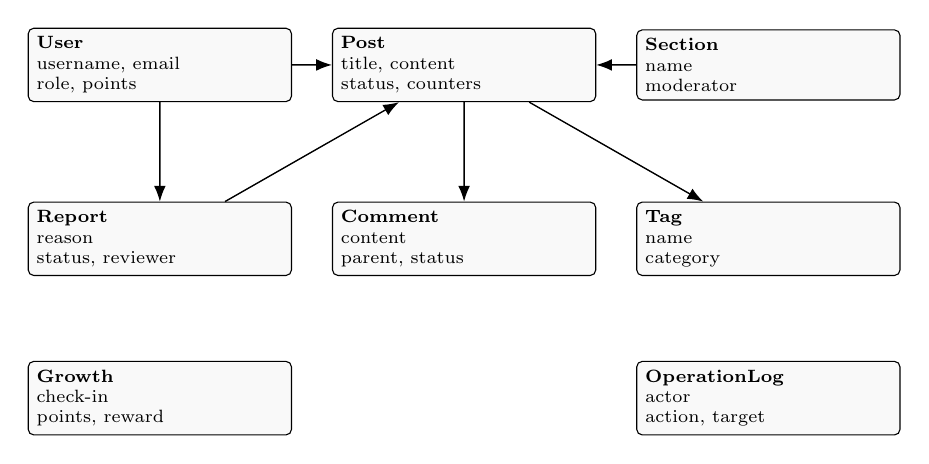
\begin{tikzpicture}[x=1cm,y=1cm,scale=0.92,transform shape]
\node[classbox] (user) at (0,2.6) {\textbf{User}\\username, email\\role, points};
\node[classbox] (post) at (4.2,2.6) {\textbf{Post}\\title, content\\status, counters};
\node[classbox] (section) at (8.4,2.6) {\textbf{Section}\\name\\moderator};
\node[classbox] (report) at (0,0.2) {\textbf{Report}\\reason\\status, reviewer};
\node[classbox] (comment) at (4.2,0.2) {\textbf{Comment}\\content\\parent, status};
\node[classbox] (tag) at (8.4,0.2) {\textbf{Tag}\\name\\category};
\node[classbox] (growth) at (0,-2.0) {\textbf{Growth}\\check-in\\points, reward};
\node[classbox] (log) at (8.4,-2.0) {\textbf{OperationLog}\\actor\\action, target};

\draw[arr] (user) -- (post);
\draw[arr] (section) -- (post);
\draw[arr] (post) -- (tag);
\draw[arr] (post) -- (comment);
\draw[arr] (user) -- (report);
\draw[arr] (report) -- (post);
\end{tikzpicture}
\caption{西南交大校园论坛系统简化类图}
\end{figure}

该逻辑模型体现了论坛系统的四条主线：用户围绕版块发布帖子，帖子产生评论、标签和浏览互动；用户对内容进行点赞、收藏、举报和不感兴趣反馈；签到、积分流水、奖励项和兑换申请构成成长体系；管理员和版主通过举报、帖子状态、用户状态和操作日志完成治理闭环。

\paragraph{开发及运行视图设计}

开发视图对应代码组织方式。前端位于 \texttt{frontend/}，包含页面 HTML、共享运行时和样式；后端位于 \texttt{backend/}，核心包名为 \texttt{com.swjtu.forum}，按 controller、service、repository、entity、dto、security、exception、config 组织。运行视图关注一次真实请求如何穿越各层。

\begin{figure}[H]
\centering
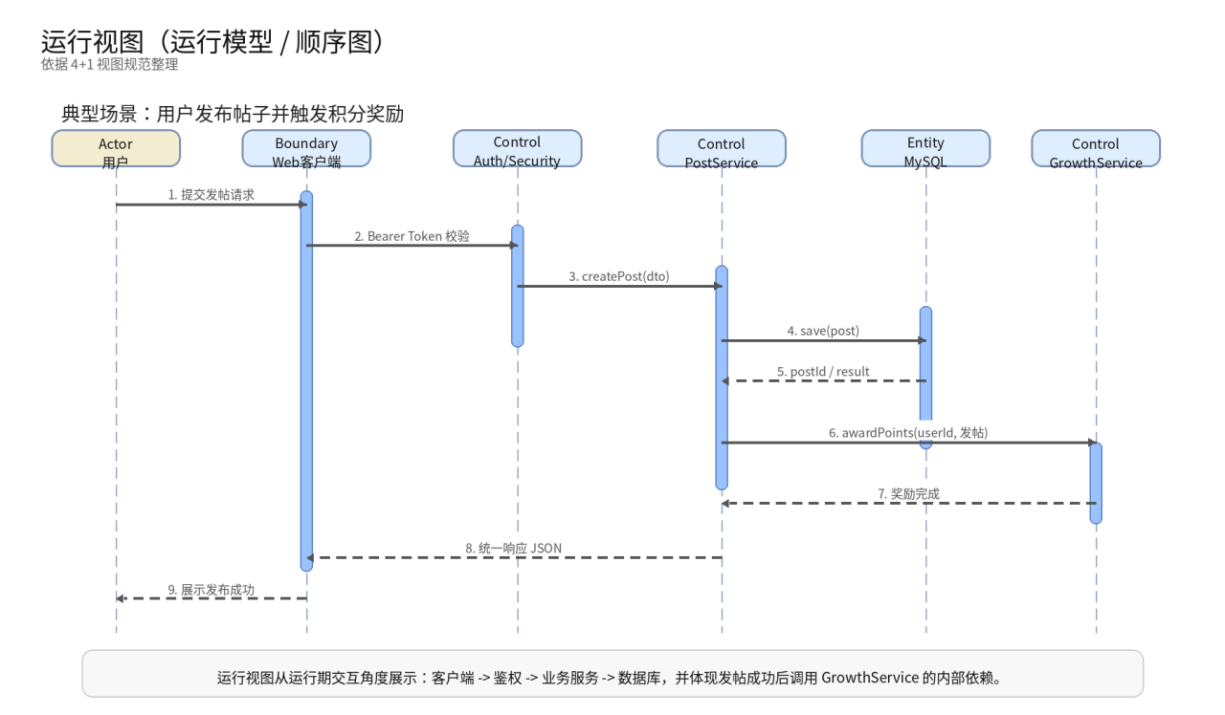
\includegraphics[width=0.95\linewidth]{media/media/image4.png}
\caption{系统开发及运行视图}
\end{figure}

以“用户发布帖子”为例，浏览器在发帖页提交标题、正文、版块和标签；前端运行时从会话中取出 JWT 并调用 \texttt{POST /api/posts}；JWT 过滤器解析用户身份；\texttt{PostController} 校验 \texttt{PostRequest} 后调用 \texttt{PostService}；业务层校验用户状态、版块存在性、内容长度和标签；Repository 写入 \texttt{posts} 与 \texttt{post\_tags}；成功后返回统一响应。若校验失败或权限不足，异常处理器返回 400、401、403 或业务错误信息，前端保留用户输入并展示友好提示。

\paragraph{部署视图设计}

部署视图描述系统交付后的节点、执行环境和通信关系。正式部署时，前端静态资源由 Web 服务器或 Vite 构建产物托管，后端以 Spring Boot Jar 运行，数据库使用 MySQL 8；Redis 作为可选缓存与短期状态扩展点。本地演示时可使用 H2 文件数据库替代 MySQL。

\begin{figure}[H]
\centering
\begin{tikzpicture}[node distance=10mm and 14mm, scale=0.88, transform shape]
\node[box, text width=30mm, fill=blue!6] (client) {用户终端\\Chrome/Edge};
\node[box, text width=34mm, fill=gray!8, right=of client] (web) {前端节点\\Vite dist\\HTML/CSS/JS};
\node[box, text width=38mm, fill=gray!8, right=of web] (app) {应用服务器\\JDK 17\\forum-1.0.0.jar};
\node[db, below=of app] (mysql) {MySQL 8\\swjtu\_forum};
\node[db, left=of mysql] (redis) {Redis\\缓存扩展};
\node[db, right=of mysql] (h2) {H2\\演示数据};

\draw[arr] (client) -- node[above,font=\scriptsize]{HTTPS} (web);
\draw[arr] (web) -- node[above,font=\scriptsize]{/api JSON} (app);
\draw[arr] (app) -- node[right,font=\scriptsize]{JDBC} (mysql);
\draw[arr,dashed] (app) -- node[above,font=\scriptsize]{可选} (redis);
\draw[arr,dashed] (app) -- node[above,font=\scriptsize]{demo/local profile} (h2);
\end{tikzpicture}
\caption{系统部署图}
\end{figure}

部署图中，前端和后端通过 HTTP/HTTPS 与 JSON 通信，后端与数据库通过 JDBC 通信。正式环境建议将 JWT 密钥、数据库用户名、数据库密码等配置放入环境变量；演示环境默认使用本地 H2 文件数据库和初始化数据，使答辩时即使没有 MySQL 服务也能展示核心功能流程。

部署时建议区分开发、演示和正式三个运行环境。开发环境以 Vite dev server 和后端本地端口联调用于快速调试；演示环境通过 H2 初始化数据，在无外部依赖的情况下展示注册、发帖、评论、签到、兑换和后台审核；正式环境使用 MySQL 8，并将数据库密码、JWT 密钥、跨域白名单和日志级别放入环境变量或配置中心。后端只暴露 \texttt{/api} 接口，数据库端口不对公网开放，管理员入口通过角色权限和操作日志进行约束。

\section{接口设计}

\subsection{外部接口}

外部接口以 REST 风格提供，根路径为 \texttt{/api}。统一成功响应结构如下：\texttt{\{code: 200, message: "success", data: ...\}}。除公开浏览接口外，受保护接口需要请求头 \texttt{Authorization: Bearer <token>}。接口分组见表3-1。

\begin{longtable}{C{0.09\linewidth}L{0.28\linewidth}C{0.12\linewidth}L{0.32\linewidth}}
\caption{外部 REST 接口分组}\\
\toprule
方法 & 路径 & 权限 & 说明 \\
\midrule
\endfirsthead
\multicolumn{4}{r}{续表 \thetable}\\
\toprule
方法 & 路径 & 权限 & 说明 \\
\midrule
\endhead
\bottomrule
\endfoot
POST & \path{/api/auth/register} & 公开 & 注册用户，校验用户名、邮箱和密码格式。\\
POST & \path{/api/auth/login} & 公开 & 登录并返回 JWT。\\
GET & \path{/api/auth/me} & 登录 & 获取当前登录用户资料。\\
PUT & \path{/api/users/me} & 登录 & 更新个人资料。\\
PUT & \path{/api/users/me/campus-identity} & 登录 & 提交校园身份认证信息。\\
GET & \path{/api/sections} & 公开 & 获取版块列表。\\
POST & \path{/api/posts} & 登录 & 发布帖子。\\
GET & \path{/api/posts} & 公开 & 分页获取公开帖子。\\
GET & \path{/api/posts/hot} & 公开 & 获取热门帖子。\\
GET & \path{/api/posts/search} & 公开 & 按关键词搜索帖子。\\
GET & \path{/api/posts/recommend} & 可选登录 & 获取推荐帖子，登录用户结合兴趣标签。\\
GET & \path{/api/posts/mine} & 登录 & 获取我的帖子。\\
GET & \path{/api/posts/favorites} & 登录 & 获取我的收藏。\\
GET & \path{/api/posts/history} & 登录 & 获取浏览记录。\\
GET & \path{/api/posts/{id}} & 公开 & 获取帖子详情。\\
PUT & \path{/api/posts/mine/{id}} & 作者 & 编辑自己的帖子。\\
POST & \path{/api/posts/{id}/like} & 登录 & 点赞或取消点赞帖子。\\
POST & \path{/api/posts/{id}/favorite} & 登录 & 收藏或取消收藏帖子。\\
POST & \path{/api/posts/{id}/report} & 登录 & 举报帖子。\\
GET & \path{/api/posts/{id}/comments} & 公开 & 获取帖子评论。\\
POST & \path{/api/posts/{id}/comments} & 登录 & 发布评论或回复。\\
POST & \path{/api/growth/check-in} & 登录 & 每日签到并增加积分经验。\\
GET & \path{/api/growth/points-history} & 登录 & 查询积分流水。\\
GET & \path{/api/growth/rewards} & 登录 & 查询奖励项。\\
POST & \path{/api/growth/rewards/{id}/redeem} & 登录 & 申请积分兑换。\\
GET & \path{/api/admin/posts} & ADMIN & 全站帖子管理。\\
PATCH & \path{/api/admin/posts/{id}/status} & 版主/管理员 & 审核或隐藏帖子。\\
GET & \path{/api/admin/reports} & 版主/管理员 & 查询举报列表。\\
PATCH & \path{/api/admin/reports/{id}/review} & 版主/管理员 & 处理举报。\\
GET & \path{/api/admin/users} & ADMIN & 用户列表与筛选。\\
PATCH & \path{/api/admin/users/{id}/ban} & ADMIN & 封禁用户。\\
POST & \path{/api/admin/sections} & ADMIN & 新增版块。\\
GET & \path{/api/admin/logs} & ADMIN & 查看后台操作日志。\\
PUT & \path{/api/admin/recommendations/config} & ADMIN & 更新推荐策略权重。\\
\end{longtable}

接口设计遵循四项约束：公开读取和受保护写入分离，游客可浏览公开内容但不能产生互动数据；所有写入接口使用 DTO 接收参数并通过 Bean Validation 校验；角色权限以后端注解和安全过滤器判断，前端不作为最终授权依据；所有接口返回统一结构，前端按 \texttt{code} 和 HTTP 状态决定页面提示、重试、跳转或清空会话。

统一响应结构用于降低前端适配成本。成功响应固定包含 \texttt{code}、\texttt{message} 和 \texttt{data}；分页类接口的 \texttt{data} 中包含记录列表、页码、页大小和总数；失败响应保留相同外层结构，\texttt{message} 放置可展示给用户的中文提示，内部异常细节写入后端日志。典型约定见表3-2。

\begin{longtable}{L{0.22\linewidth}L{0.28\linewidth}L{0.40\linewidth}}
\caption{外部接口统一约定}\\
\toprule
约定项 & 示例 & 设计说明 \\
\midrule
\endfirsthead
\multicolumn{3}{r}{续表 \thetable}\\
\toprule
约定项 & 示例 & 设计说明 \\
\midrule
\endhead
\bottomrule
\endfoot
鉴权头 & \path{Authorization: Bearer <token>} & 受保护接口必须携带 JWT；公开接口可不携带，推荐接口可根据是否登录返回不同结果。\\
成功响应 & \path{{code:200,message:"success",data:{...}}} & 前端统一从 \texttt{data} 取业务数据，减少各页面重复判断。\\
分页参数 & \path{page,size,keyword,status} & 列表接口统一使用页码、页大小和筛选条件，便于首页、个人中心和后台共用分页逻辑。\\
业务错误 & \texttt{code=400}，如“今日已签到” & 可预期错误使用明确中文提示，前端直接展示并保留当前输入。\\
权限错误 & \path{401/403} & 未登录跳转登录，权限不足只提示无权操作，不暴露后台接口细节。\\
\end{longtable}

\subsection{内部接口}

内部接口指后端各层之间的调用契约。Controller 只做协议适配，Service 承载业务规则，Repository 只负责持久化，Security 和 Exception 作为横切组件参与请求生命周期。表3-3 给出关键内部接口。

\begin{longtable}{L{0.30\linewidth}L{0.18\linewidth}L{0.42\linewidth}}
\caption{内部模块接口与职责}\\
\toprule
调用关系 & 形式 & 责任说明 \\
\midrule
\endfirsthead
\multicolumn{3}{r}{续表 \thetable}\\
\toprule
调用关系 & 形式 & 责任说明 \\
\midrule
\endhead
\bottomrule
\endfoot
\texttt{JwtAuthenticationFilter -> JwtUtil} & 方法调用 & 解析 Bearer Token，校验签名和过期时间，提取用户名和角色。\\
\texttt{AuthController -> UserService} & 依赖注入 & 完成注册、密码校验、用户查询和 JWT 登录上下文建立。\\
\texttt{PostController -> PostService} & 依赖注入 & 发布、查询、编辑、点赞、收藏、浏览记录、评论和帖子状态变更。\\
\texttt{GrowthController -> GrowthDiscoveryService} & 依赖注入 & 兴趣标签、签到、积分流水、奖励查询与兑换申请。\\
\texttt{AdminController -> AdminOpsService} & 依赖注入 & 用户封禁、版块维护、帖子管理、推荐策略和操作日志查询。\\
\texttt{AdminController -> ReportService} & 依赖注入 & 举报列表、举报审核、批量处理和举报统计。\\
\texttt{Service -> Repository} & JPA 接口 & 通过实体仓库读写 \texttt{users}、\texttt{posts}、\texttt{comments} 等表。\\
\texttt{Service -> OperationLogRepository} & JPA 接口 & 记录后台管理动作，支撑审计与问题追踪。\\
\texttt{GlobalExceptionHandler -> ApiResponse} & 统一封装 & 将校验异常、业务异常、资源不存在和系统异常转成可展示响应。\\
\end{longtable}

内部接口的数据流转规则为：外部请求进入 Controller 后转为 DTO，Controller 调用 Service；Service 查询或修改 Entity，并将结果组装为响应 DTO 或 Map；Repository 不直接向前端返回数据；异常统一向上抛出，由全局异常处理器转换。该规则可以避免数据库结构泄露到接口层，也便于后续将特定模块拆分为独立服务。

内部接口还规定了事务边界：Controller 和 Repository 不开启业务事务，跨表写入由 Service 方法承担；查询类方法使用只读事务，修改类方法使用普通事务。以“积分兑换”为例，业务层同时检查奖励状态、库存和用户积分，写入兑换申请，扣减或冻结积分，并记录积分流水。若任一环节失败，事务回滚，前端收到明确错误提示，数据库不保留半完成数据。

\section{系统数据库设计}

\subsection{概念数据库设计}

数据库概念设计以论坛核心业务对象为中心。主要实体包括用户、版块、帖子、评论、标签、举报、积分流水、奖励项、兑换申请、后台操作日志和推荐策略配置。用户与帖子、评论、点赞、收藏、举报、签到、兑换之间存在一对多关系；帖子与标签、用户与兴趣标签之间存在多对多关系；帖子属于版块，版块可指定版主。图4-1 给出 ER 概念模型。

\begin{figure}[H]
\centering
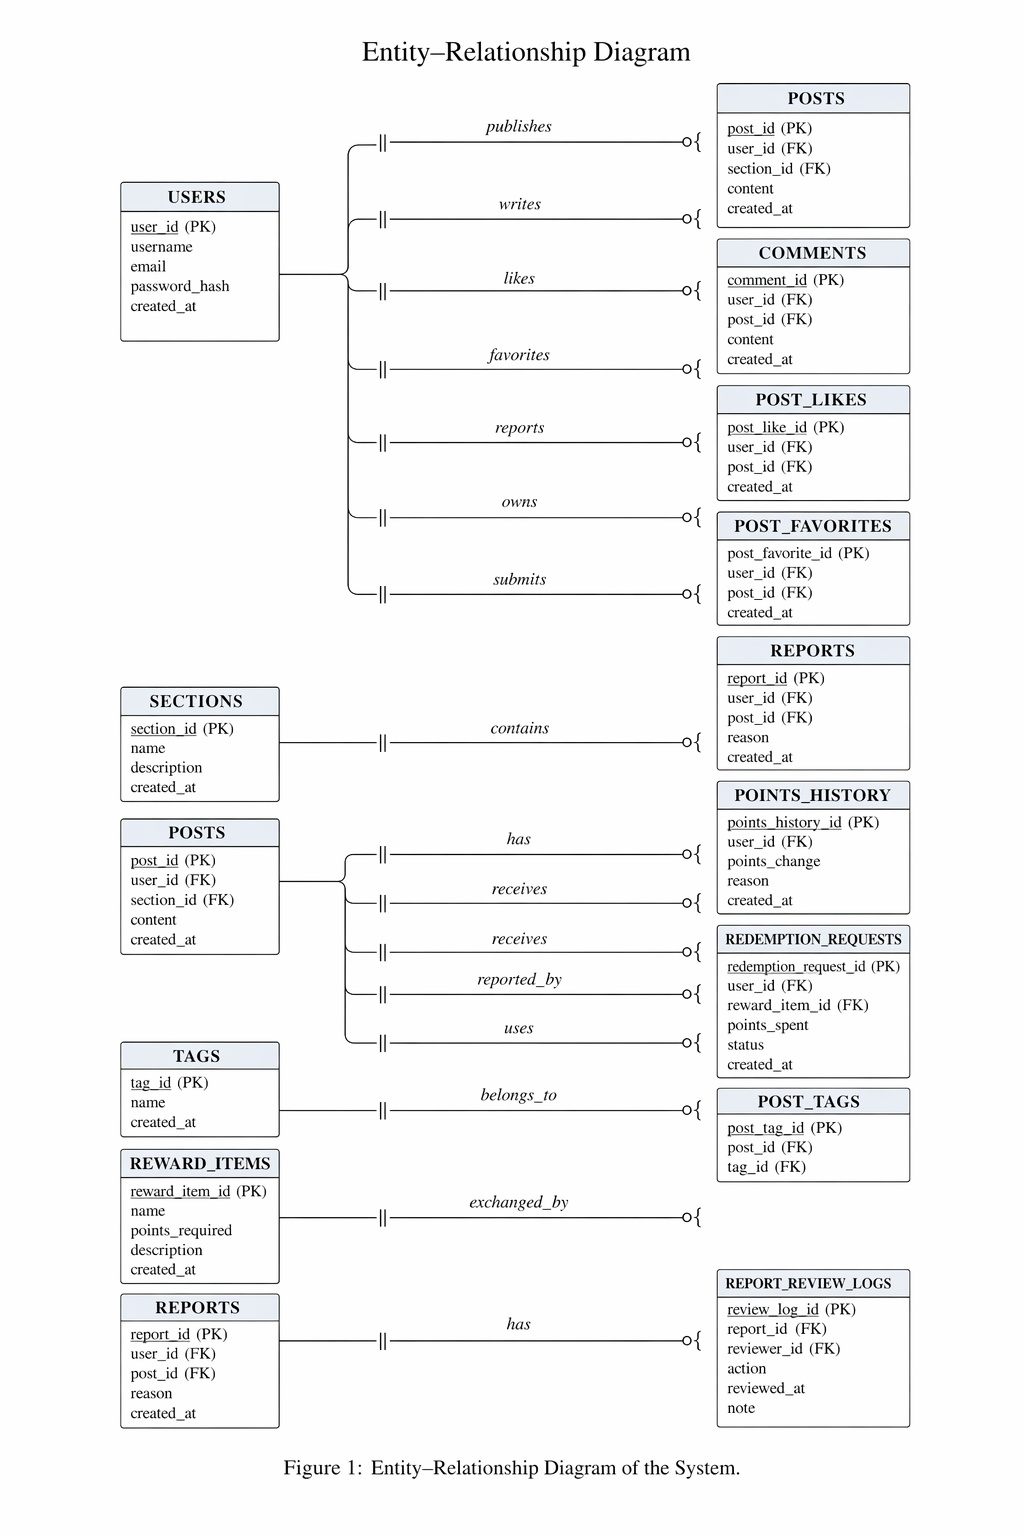
\includegraphics[width=0.74\linewidth]{media/media/image8.png}
\caption{系统数据库 ER 概念模型}
\end{figure}

概念模型中的关键联系如下：用户可以发布多个帖子，帖子必须归属于一个版块；帖子拥有多条评论，评论通过 \texttt{parent\_id} 形成回复树；帖子和标签为多对多关系，通过 \texttt{post\_tags} 关联表实现；用户和兴趣标签也是多对多关系，通过 \texttt{user\_tags} 关联表实现；点赞、收藏、浏览记录是用户与帖子之间的行为关系；举报由用户提交，指向某个帖子，并可由版主或管理员处理。

\subsection{逻辑数据库设计}

逻辑数据库设计依据 \texttt{backend/src/main/resources/schema.sql} 和 JPA 实体整理，可通过 PowerDesigner 等工具按 SQL 反向工程生成物理模型。正式数据库名为 \texttt{swjtu\_forum}，字符集为 \texttt{utf8mb4}，存储引擎为 InnoDB。核心逻辑表见表4-1。

\begin{longtable}{L{0.22\linewidth}L{0.54\linewidth}L{0.10\linewidth}}
\caption{核心逻辑表清单}\\
\toprule
表名 & 说明 & 类型 \\
\midrule
\endfirsthead
\multicolumn{3}{r}{续表 \thetable}\\
\toprule
表名 & 说明 & 类型 \\
\midrule
\endhead
\bottomrule
\endfoot
\texttt{users} & 用户账户、角色、状态、校园认证、成长积分和个人资料。 & 主表\\
\texttt{sections} & 论坛版块，包含版块描述、排序、帖子数缓存和版主外键。 & 主表\\
\texttt{tags} & 标签字典，支持帖子标签和用户兴趣标签。 & 字典表\\
\texttt{posts} & 帖子主表，保存标题、正文、版块、作者、状态、热度和统计字段。 & 主表\\
\texttt{comments} & 评论表，支持父评论形成回复链，支持隐藏状态。 & 主表\\
\path{post_tags} & 帖子与标签的多对多关系表。 & 关联表\\
\path{user_tags} & 用户兴趣标签多对多关系表。 & 关联表\\
\path{post_likes} & 帖子点赞关系，限制同一用户对同一帖子只能点赞一次。 & 行为表\\
\path{comment_likes} & 评论点赞关系，限制重复点赞。 & 行为表\\
\path{post_favorites} & 帖子收藏关系，限制重复收藏。 & 行为表\\
\path{post_browse_history} & 帖子浏览记录，保留首次浏览和最近浏览时间。 & 行为表\\
\texttt{reports} & 帖子举报主表，记录举报原因、处理人、状态和审核备注。 & 治理表\\
\path{report_review_logs} & 举报处理历史，保留每次审核动作。 & 治理表\\
\path{operation_logs} & 管理员/版主操作日志，用于审计和故障追溯。 & 审计表\\
\path{daily_checkins} & 每日签到记录，按用户和日期唯一。 & 成长表\\
\path{points_history} & 积分和经验变更流水。 & 成长表\\
\path{reward_items} & 积分商城奖励项。 & 成长表\\
\path{redemption_requests} & 积分兑换申请与审核状态。 & 成长表\\
\path{recommendation_configs} & 推荐策略权重配置。 & 配置表\\
\end{longtable}

主键统一采用 \texttt{BIGINT AUTO\_INCREMENT}。外键约束用于保证帖子必须关联有效用户和版块，评论必须关联有效帖子和用户，举报必须关联有效帖子和举报人。对可能重复提交的行为表建立联合唯一约束，例如帖子点赞、帖子收藏、浏览记录和每日签到均按“用户 + 业务对象”唯一。常用查询字段建立组合索引，例如帖子按“版块、状态、创建时间”索引，举报按“状态、创建时间”索引，用于支撑首页、个人中心、后台审核和举报列表分页。关键约束与索引见表4-2。

\begin{longtable}{L{0.25\linewidth}L{0.24\linewidth}L{0.41\linewidth}}
\caption{关键数据库约束与索引设计}\\
\toprule
对象 & 约束或索引 & 设计目的 \\
\midrule
\endfirsthead
\multicolumn{3}{r}{续表 \thetable}\\
\toprule
对象 & 约束或索引 & 设计目的 \\
\midrule
\endhead
\bottomrule
\endfoot
\texttt{users} & 用户名、邮箱唯一 & 防止重复注册，保证登录标识唯一。\\
\texttt{posts} & \path{idx_posts_section_status_created} & 支撑按版块、状态和时间分页查询帖子。\\
\texttt{comments} & \path{idx_comments_post_status_created} & 支撑帖子详情页按时间加载可见评论。\\
\path{post_tags} & \path{PRIMARY KEY(post_id, tag_id)} & 保证同一帖子不重复绑定同一标签。\\
\path{post_likes} & \path{uk_post_likes_user_post} & 保证同一用户对同一帖子只能形成一条点赞关系。\\
\path{post_favorites} & \path{uk_post_favorites_user_post} & 保证收藏操作幂等，避免重复收藏。\\
\path{post_browse_history} & \path{uk_post_browse_history_user_post} & 合并同一用户的重复浏览，只更新最近浏览时间。\\
\path{daily_checkins} & \path{UNIQUE(user_id, check_date)} & 保证用户每天只能签到一次，避免重复发放积分和经验。\\
\texttt{reports} & \path{idx_reports_status_created} & 支撑后台按待处理、已处理状态分页审核。\\
\path{operation_logs} & \path{idx_operation_logs_target} & 支撑按对象类型和对象 ID 追踪管理员动作。\\
\end{longtable}

数据库逻辑设计可导出为建库脚本。初始化入口命名为 \texttt{init-database.sql}，完整建表脚本命名为 \texttt{backend/src/main/resources/schema.sql}。正式部署时可执行建库脚本创建 \texttt{swjtu\_forum} 数据库；演示环境可使用 H2 自动初始化相同核心表结构。该设计满足课程要求中“导出 SQL，创建数据库”的交付要求，并为后续实现和部署验证提供依据。

\section{系统出错处理设计}

\subsection{出错信息}

系统错误处理采用“后端统一响应，前端友好提示”的策略。后端通过 Spring Security、Bean Validation 和 \texttt{GlobalExceptionHandler} 将异常转换为标准响应；前端运行时根据状态码决定弹窗、表单提示、跳转登录或保留输入。表5-1 列出主要错误场景。

\begin{longtable}{C{0.08\linewidth}L{0.16\linewidth}L{0.19\linewidth}L{0.17\linewidth}L{0.20\linewidth}}
\caption{系统出错信息一览表}\\
\toprule
状态 & 场景 & 输出信息 & 含义 & 前端提醒方式 \\
\midrule
\endfirsthead
\multicolumn{5}{r}{续表 \thetable}\\
\toprule
状态 & 场景 & 输出信息 & 含义 & 前端提醒方式 \\
\midrule
\endhead
\bottomrule
\endfoot
400 & 注册参数不合法 & 参数校验失败 & 用户名、邮箱、密码或正文长度不满足约束。 & 在表单字段旁显示错误，保留已输入内容。\\
400 & 重复注册 & 用户名或邮箱已存在 & 唯一约束或业务校验失败。 & 提示更换用户名或邮箱。\\
401 & 未登录访问写接口 & 请先登录后再操作 & 请求未携带 JWT 或 JWT 无效。 & 清除无效会话，引导到登录页并记录回跳地址。\\
401 & Token 过期 & 登录状态已过期，请重新登录 & JWT 超时或签名校验失败。 & 弹出登录过期提示，保留当前页面状态。\\
403 & 权限不足 & 当前账号无权执行该操作 & 普通用户访问后台接口或越权修改他人帖子。 & 显示无权限提示，不暴露接口细节。\\
404 & 帖子不存在 & 资源不存在 & 请求 ID 不存在或内容已删除。 & 展示空状态，并提供返回列表按钮。\\
409 & 重复点赞或签到 & 请勿重复操作 & 数据库唯一约束或业务状态阻止重复提交。 & 按当前真实状态刷新按钮。\\
422 & 内容审核失败 & 内容包含不适宜发布的信息 & 敏感词或状态规则阻止发布。 & 保留草稿并突出需修改内容。\\
500 & 数据库连接异常 & 服务暂时不可用，请稍后重试 & MySQL 不可用、连接池耗尽或底层异常。 & 显示统一服务维护提示，允许稍后重试。\\
500 & 未预期系统异常 & 系统繁忙，请稍后再试 & 未分类运行时异常。 & 记录日志，前端显示通用错误页或通知。\\
\end{longtable}

\subsection{补救措施}

故障补救以“尽量保护用户输入，尽快恢复服务，保留审计证据”为原则。

\Needspace{10\baselineskip}
\begin{center}
\begin{minipage}{0.88\linewidth}
\algcaption{统一出错处理流程}
{\zihao{5}
\begin{enumerate}
\item 前端发起请求前检查必填字段、网络状态和本地登录状态。
\item 后端安全过滤器解析 JWT，若无效则返回 401，若角色不足则返回 403。
\item Controller 将请求参数转换为 DTO，并执行格式、长度和必填项校验。
\item Service 执行业务规则校验，涉及多表写入时开启事务。
\item Repository 持久化数据，数据库外键、唯一约束和索引保证数据边界。
\item 若任一环节失败，异常交给 \texttt{GlobalExceptionHandler} 转换为统一响应。
\item 前端根据状态码展示字段提示、Toast、登录跳转或空状态，并保留可恢复输入。
\item 后端记录必要日志，管理员可通过操作日志和举报审核日志追踪问题。
\end{enumerate}
}
\end{minipage}
\end{center}

\term{前端补救。} 对发帖、评论、资料编辑等表单操作，前端在提交失败时不清空输入；对 Token 失效，清理本地身份信息并跳转登录，登录成功后回到原页面；对后台列表操作失败，保留筛选条件、分页和勾选状态，避免管理员重复定位。

\term{后端补救。} 对可预期业务错误使用明确异常，例如资源不存在、权限不足、重复操作和参数校验失败；对积分兑换、帖子状态修改、举报审核等涉及多表更新的操作设置事务边界，失败时回滚，避免部分成功；管理员操作写入 \texttt{operation\_logs}，举报处理写入 \texttt{report\_review\_logs}，便于事后追踪。

\term{数据库补救。} 对点赞、收藏、浏览记录和签到等幂等性敏感操作使用唯一约束兜底；对帖子、评论、互动、标签关系等依赖关系使用外键和级联删除，避免孤立数据；正式部署时建议定时备份 \texttt{swjtu\_forum}，遇到误删或故障时结合操作日志恢复到最近一致状态。

\term{部署补救。} 如果正式 MySQL 不可用，课程演示可临时切换到 H2 本地 profile 完成主要功能展示；如果前端请求失败，优先检查后端 8080 端口、Vite 代理和 \texttt{/api} 根路径；如果权限异常集中出现，优先检查 JWT 密钥、系统时间和用户角色字段。

\end{document}
